\section{No Analytic Solution for Inference-Compute Optimality} \label{sec:proof1}
In this section, we prove that it is not possible to analytically derive the optimal model size and pre-training token count according to the third Chinchilla law, after accounting for the computational cost of inference. Conditioned on model quality, we assume that inference demand does not depend on model size and can be estimated prior to training.

\begin{theorem}
\label{noanalytic}
Given a fixed model quality and inference demand, there exists no general analytic solution for the compute-optimal model size and pre-training token count according to the third Chinchilla law, after accounting for the computational cost of inference. 
\end{theorem}
\begin{proof}
By Eq. \ref{eq:2}, the overall compute cost in FLOPs for training a model with $N$ parameters on $\Dtr$ tokens and running inference on $\Dinfi$ tokens is given by $C(N, \Dtr, \Dinfi) = 6N\Dtr + 2N\Dinfi$. 

We seek the minimum overall compute budget to train and deploy a model of a given quality and inference demand. Formally, we optimize the objective:
\begin{align}
\min C(N, \Dtr, \Dinfi)
\end{align}
subject to the constraint
$L(N, \Dtr) =  E + \frac{A}{N^\alpha} + \frac{B}{D_{\text{tr}}^\beta} = \ell$.

This constraint, from the third Chinchilla law, ensures we are minimizing compute while fixing model quality (pre-training loss). $A = 406.4, B = 410.7, E = 1.69, \alpha = 0.336$, and $\beta = 0.283$ are constants determined empirically by \citet{chinchilla}.\footnote{The Chinchilla paper reports $\alpha = 0.34$ and $\beta = 0.28$. However, these are rounded values; to better fit the results reported in Table A.3 of \citet{chinchilla}, we use $\alpha = 0.336$ and $\beta = 0.283$, as in \citet{blogpost}.}

We solve this optimization problem via the method of Lagrange multipliers. The gradients are:
\begin{align}
\nabla C(N, \Dtr) = (6D + 2\Dinfi) \hat{i} + 6N \hat{j}
\end{align}
\begin{align}
\nabla L(N, \Dtr) = -\alpha A N^{-\alpha - 1}\hat{i} - \beta B \Dtr ^{-\beta - 1} \hat{j}
\end{align}
We have three equations and three variables ($\Dtr, N, \lambda$), where $\lambda$ is our Lagrange multiplier:
\begin{align}
6\Dtr + 2\Dinfi  = -\lambda \alpha A N^{-\alpha - 1} &&
6N = -\lambda \beta B \Dtr ^{-\beta - 1}
&&
E + \frac{A}{N^\alpha} + \frac{B}{\Dtr^{\beta}} = \ell
\end{align}
With some algebraic manipulation, we can eliminate $\lambda$ and write $\frac{A}{N^\alpha}$ in terms of $\Dtr$:
\begin{align}
\frac{A}{N^{\alpha}} = \frac{3\beta B \Dtr^{-\beta} + \Dinfi \beta B \Dtr^{-\beta-1}}{3\alpha}    
\end{align}
We are left to solve the following equation for $\Dtr$: 
\begin{align}\label{eq:11}
0 = (E - \ell) + \Big[\frac{\beta B}{\alpha} + B\Big] \Dtr^{-\beta} + \frac{\Dinfi \beta B}{3\alpha}\Dtr^{-\beta-1}
\end{align}
Thus, determining $\Dtr$ as a function of $\Dinfi$ and $\ell$ involves finding the roots of equations of the form $ ax^{-1.283} + 756.6x^{-0.283} + c = 0$ for arbitrary $a$ and $c > 0$, which is not possible in general.

The best-fit constants $A, B, E, \alpha$ and $\beta$ vary based on the exact dataset and model architecture. Outside of a handful of special-case values of $\beta$ for which Eq. \ref{eq:11} can be manipulated into a low-degree polynomial, it is intractable.  
\end{proof}

\section{Further Results}
\subsection{Compute-Optimal Results}\label{sec:compoptappendix}
We present further results from our analysis in Sec. \ref{sec:compopt}. In Table \ref{table:computetable}, we show the computational cost (in FLOPs) to train and run inference for Chinchilla-style models of various sizes and inference demands. We then calculate the \textit{compute-optimal} model configuration to reach the same quality (equal loss) and run inference, and note the overall compute reduction.

\begin{table}
  \caption{Compute-Optimal vs. Chinchilla-style Models for Selected Configurations.}
  \label{table:computetable}
  \centering
  \begin{tabular}{llccccccr}
    \toprule
    & & & & & & & \\
    & & \multicolumn{3}{c}{Chinchilla Model} & \multicolumn{3}{c}{Compute-Optimal Model} \\
    \cmidrule(r){3-5} \cmidrule(r){6-8}
    Inference & Train & & Training &  &  & Training &  & FLOP
    \\ Tokens & Loss & Params & Tokens & FLOPs & Params & Tokens & FLOPs & Reduction\\
    \midrule
    50B & 2.53 & 1B & 27.4B  & 2.64e20 & 6.33M  & 46.8B & 2.41e20 & 9.1\%\\
    200B & 2.13 & 7B & 276B &  1.44e22   & 5.4B & 367B & 1.40e22 & 2.6\%    \\
    1T & 2.05 & 13B & 577B & 7.10e22 & 8.32B & 967B & 6.49e22 & 8.5\% \\
    5T & 1.96 & 30B & 1.56T  & 5.80e23 & 16.4B & 3.27T & 4.86e23 & 16\% \\
    10T & 1.89 & 70B     & 4.26T & 3.19e24 & 41.6B & 7.92T & 2.81e24 & 12\% \\
    \bottomrule
  \end{tabular}
\end{table}

\subsection{Cost-Optimal Results}\label{sec:costoptappendix}
We show additional results from our cost-optimality analysis in Sec. \ref{sec:costopt}. In Table \ref{table:costtable}, we show the total training plus inference costs for Chinchilla models of various sizes at different levels of inference demands. We then calculate costs for equivalent-quality (i.e. same pre-training loss) \textit{cost-optimal} models and show the overall savings. We use the same settings from Figure \ref{fig:cost}, designed to mimic a typical real-world deployment: training and inference input at 50\% MFU, generation at 1\% MFU \cite{megatronlm, palminference}. Each inference request has 70 input tokens and 215 output tokens, in accordance with averages from the 
LMSYS-Chat dataset of 1M inference requests from \citet{lmsys}. Costs are calculated assuming training and inference on A100-80GB and A100-40GB accelerators, respectively. We further assume the model parameters are quantized to eight-bit integers prior to inference, which is commonly done with no quality reduction \cite{smoothquant}. All costs are reported in US dollars.


\begin{table}
  \caption{Cost-Optimal vs. Chinchilla-style Models for Selected Configurations.}
  \label{table:costtable}
  \centering
  \begin{tabular}{llccccccr}
    \toprule
    & & & & & & & \\
    & & \multicolumn{3}{c}{Chinchilla Model} & \multicolumn{3}{c}{Cost-Optimal Model} \\
    \cmidrule(r){3-5} \cmidrule(r){6-8}
    Inference & Train & & Training & Total  &  & Training & Total  & Cost
    \\ Requests & Loss & Params & Tokens & Cost (\$) & Params & Tokens & Cost (\$) & Savings\\
    \midrule
    175M & 2.53 & 1B & 27.4B  & 3.77K & 327M  & 152B &  1.89K & 50\% \\
    702M & 2.13 & 7B & 276B & 124K     & 2.90B & 929B  & 81.8K & 34\%    \\
    3.51B & 2.05 & 13B & 577B & 987K & 430B & 3.1T & 500K & 49\% \\
    17.5B & 1.96 & 30B & 1.56T & 10.8M & 8.58B & 12.1T & 4.52M & 58\% \\
    35.1B & 1.89 & 70B & 4.26T & 51.5M & 21.5B & 27T & 23.8M & 54\% \\
    \bottomrule
  \end{tabular}
\end{table}

\subsection{GPU Details}\label{sec:pricing}
GPU pricing varies based on vendor and fluctuates over time. At the time of writing, an A100-40GB costs USD \$1.10/hr and an A100-80GB costs \$1.50/hr on Lambda Labs \cite{lambdalabs}. We use these values in our cost analysis in Sec. \ref{sec:costopt} and in Table \ref{table:costtable}. Both variants have a peak performance of $3.12 \times 10^{14}$ dense FP16/BF16 operations and  $6.24 \times 10^{14}$ INT8 operations per second \cite{a100datasheet}.

\section{Model Training}\label{sec:traindetails}
We train MPT-style transformer models \cite{mpt} ranging in size from 150M to 6B parameters, on token/parameter ratios from 10 to 10,000. In Table \ref{table:traintable}, we provide training configuration details. All models were trained with ALiBi \cite{alibi}, Grouped Query Attention \cite{gqa}, the Lion optimizer \cite{lion} ($\beta_1 = 0.9, \beta_2 = 0.95$) with weight decay equal to the learning rate, cosine warmup ($\alpha_f = 0.1$) with a duration equal to 3 times the number of model parameters, and norm gradient clipping (threshold = 1). A maximum sequence length of 4096 tokens was used. 
A smaller batch size was used for smaller models so that low-token-count training runs see enough update steps to learn properly. For all experimental results in this work, we use the smoothed final training loss over the last ten batches to reduce noise from minor batch-level variations.

In the rightmost column of Table \ref{table:traintable}, we list our experiment training token ratios. Note that for the larger models, our training durations are limited by our computational resources.

\begin{table}
  \caption{Model Training Configurations.}
  \label{table:traintable}
  \centering
  \begin{tabular}{llccccccr}
    \toprule
    Name & Params & d\_model & n\_heads & n\_layers & Learning Rate & Batch Size & Tokens/Parameter \\
    \midrule
    150M & 151M & 768 & 12  & 12 & 4.603e-4 & 160\tablefootnote{The 10,000 token/parameter 150M model was trained with batch size 960 due to compute issues.} & 10,15,20,30,50,75,100, & \\
    & & & & & & & 250,500,1000,5000,10000 \\
    370M & 367M & 1024 & 16 & 24 & 3.453e-4 & 320 & 10,15,20,30,50,75,100, \\
     & & & & & & &250,500,1000 \\
    750M & 749M & 1536 & 12 & 24 & 2.302e-4 & 480 & 10,15,20,30,50,75,100,250,500 \\
    1.3B & 1.26B & 2048 & 16 & 24 & 1.726e-4 & 960 & 10,15,20,30,50,75,100,250\\
    2.5B & 2.46B & 2560 & 20 & 32 & 1.381e-4 & 960 & 10,15,20,50,100,250,500 \\
    6B &  6.05B & 4096 & 32 & 32 & 8.632e-5 & 960 & 20 \\
    \bottomrule
  \end{tabular}
\end{table}


\section{Experiment Results}
\label{sec:furtherresults}
We present more results from our experiments described in Section \ref{sec:experiments}. In Figure \ref{fig:gauntletcategories}, we show aggregate results for each Gauntlet category. Within each category, every task (the tasks are enumerated in Sec. \ref{sec:experiments}) is weighted equally and averaged after subtracting out baseline and normalizing so the maximum achievable accuracy is 1. Note that for some categories (e.g. Symbolic Problem Solving), all models achieve nearly zero performance on all tasks, resulting in low correlation between accuracy and token/parameter ratios (see \citet{Barton2024}).

\begin{figure}
        \begin{subfigure}[b]{0.33\textwidth}
                \centering
                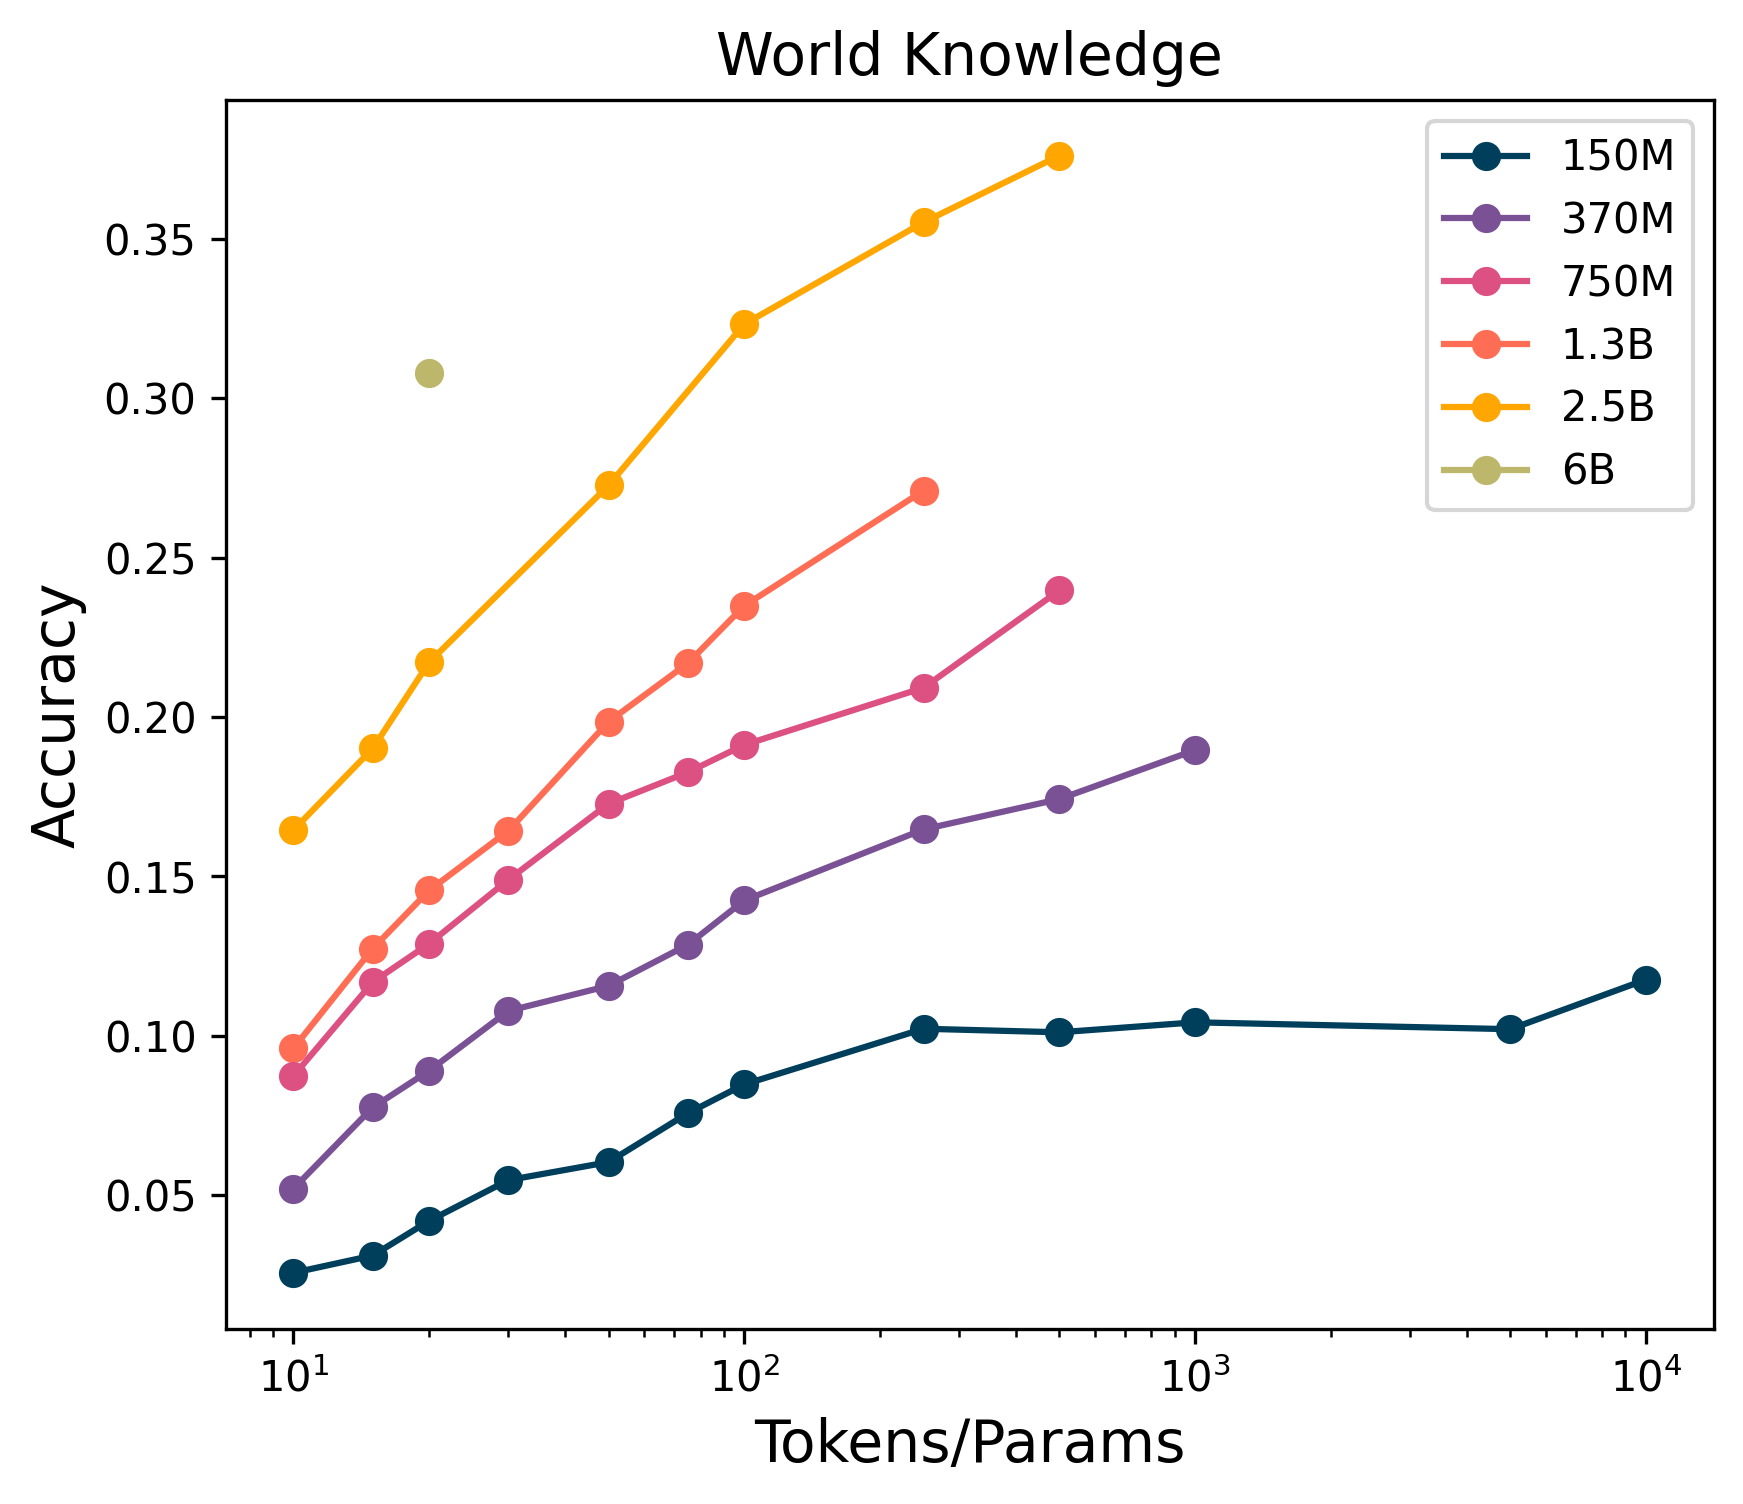
\includegraphics[width=1.00\linewidth]{figs_camera/World_Knowledge_vs_TokensParams.png}
                \caption{}
                \label{fig:worldknowledge}
        \end{subfigure}%
        \begin{subfigure}[b]{0.33\textwidth}
                \centering
                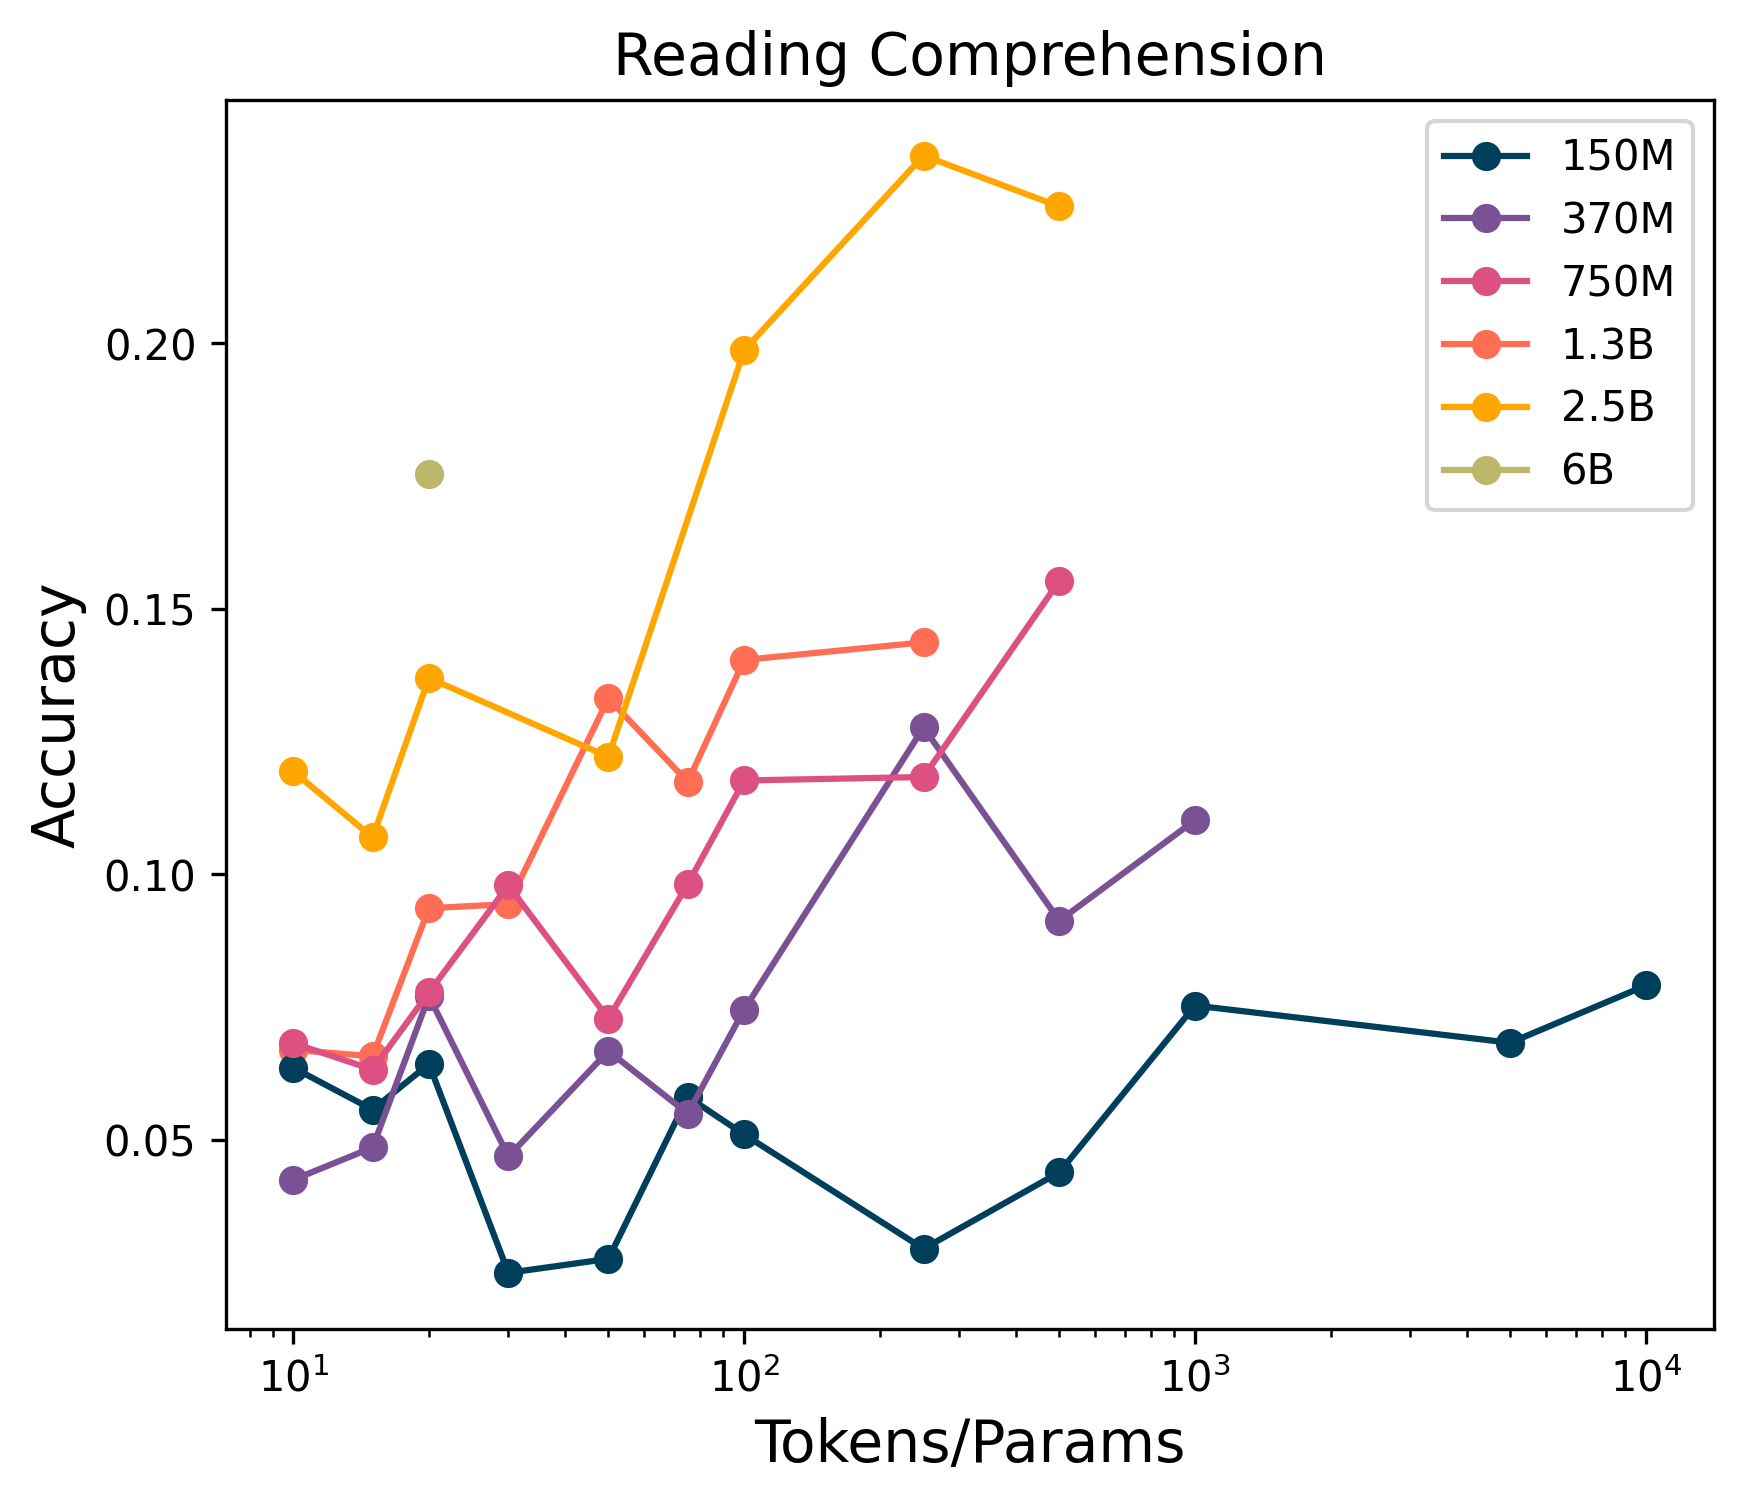
\includegraphics[width=1.00\linewidth]{figs_camera/Reading_Comprehension_vs_TokensParams.png}
                \caption{}
                \label{fig:readingcomprehension}
        \end{subfigure}%
        \begin{subfigure}[b]{0.33\textwidth}
                \centering
                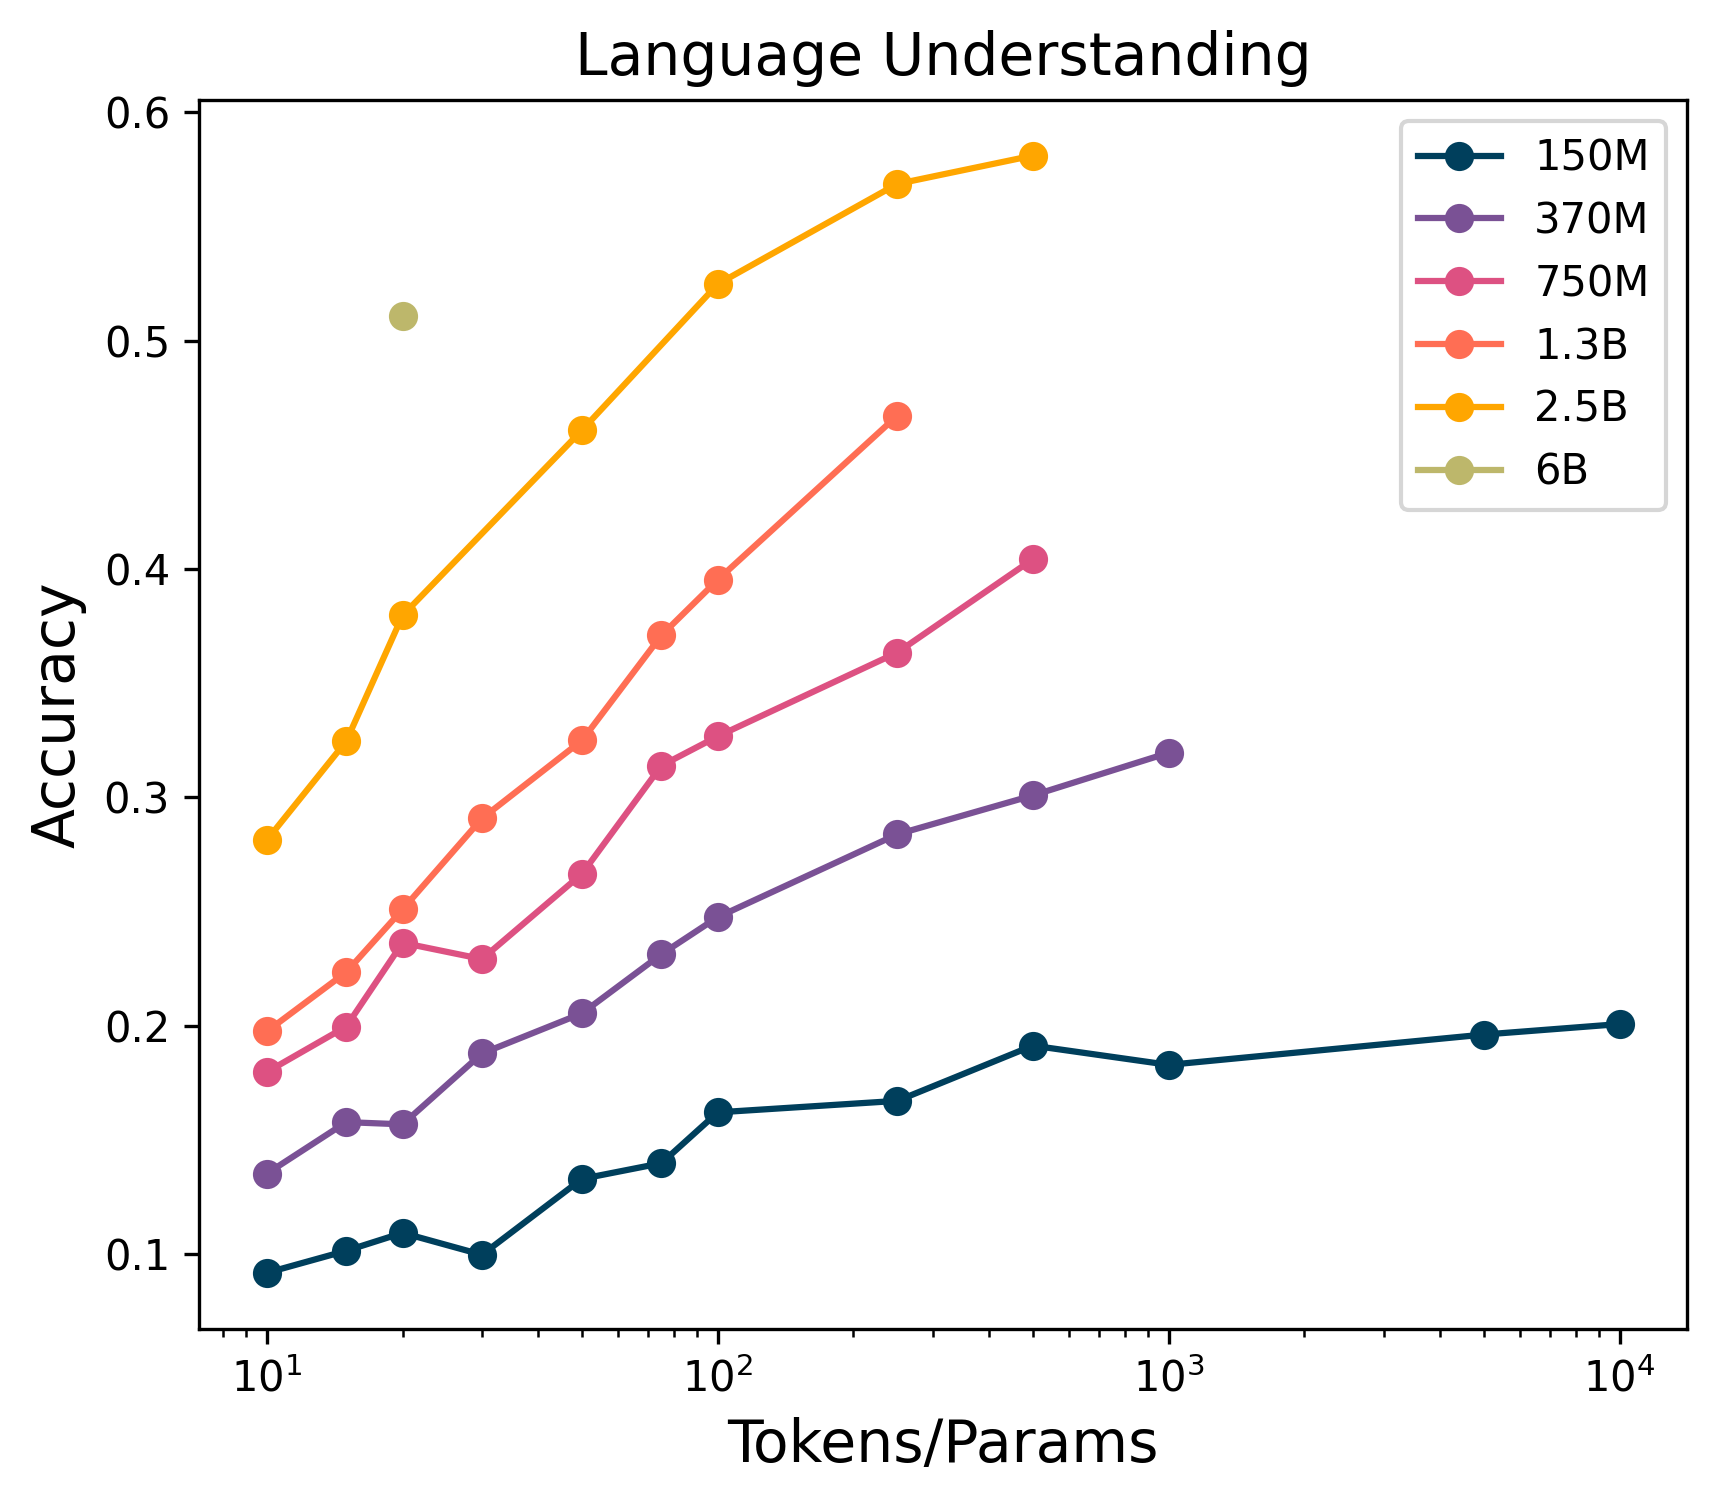
\includegraphics[width=1.00\linewidth]{figs_camera/Language_Understanding_vs_TokensParams.png}
                \caption{}
                \label{fig:languageunderstanding}
        \end{subfigure}%

        \begin{subfigure}[b]{0.33\textwidth}
                \centering
                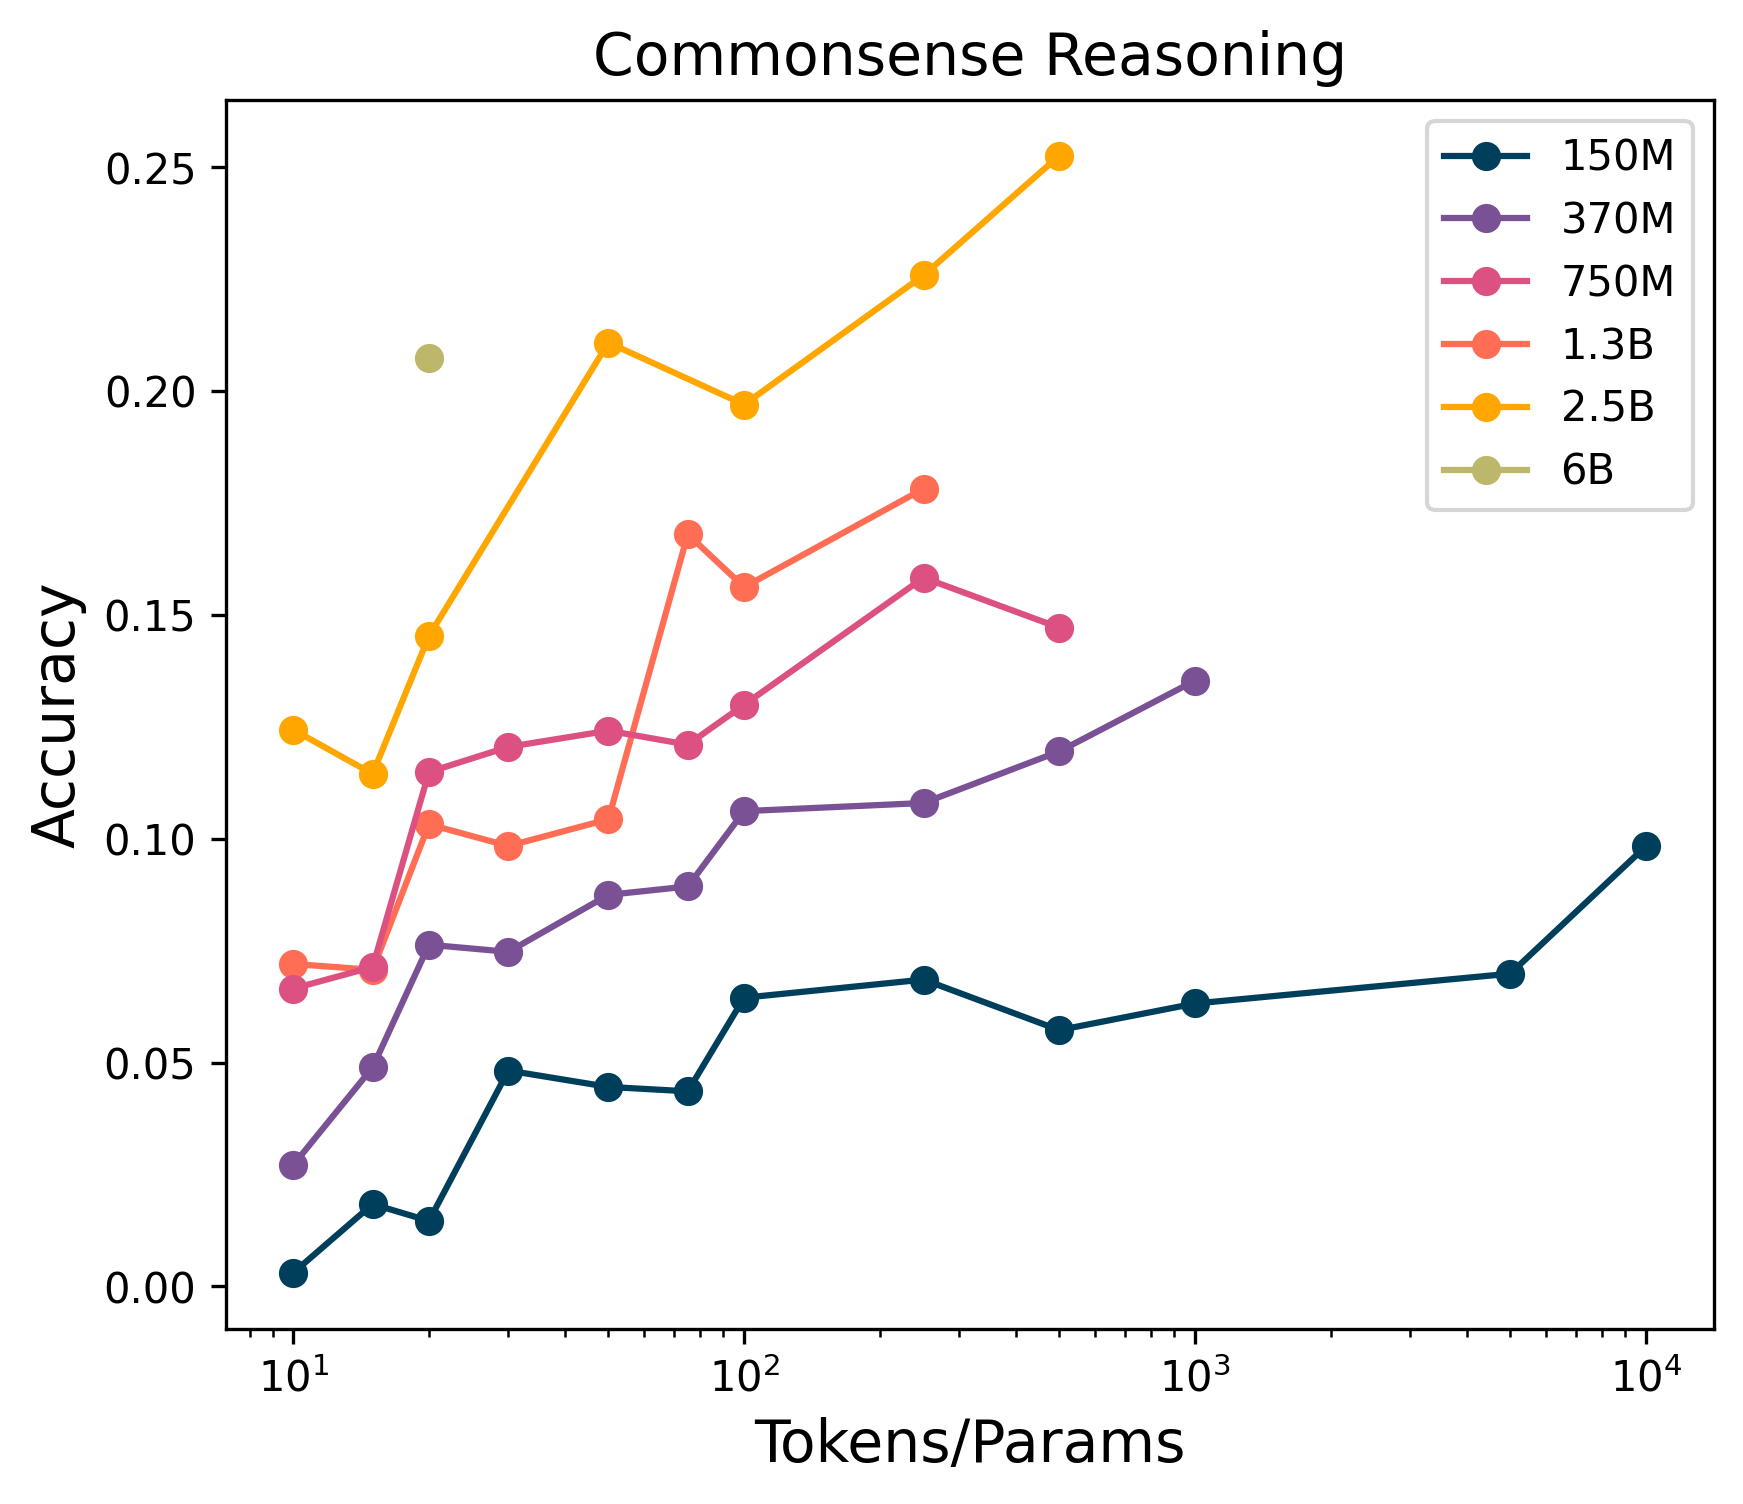
\includegraphics[width=1.00\linewidth]{figs_camera/Commonsense_Reasoning_vs_TokensParams.png}
                \caption{}
                \label{fig:commonsensereasoning}
        \end{subfigure}%
        \begin{subfigure}[b]{0.33\textwidth}
                \centering
                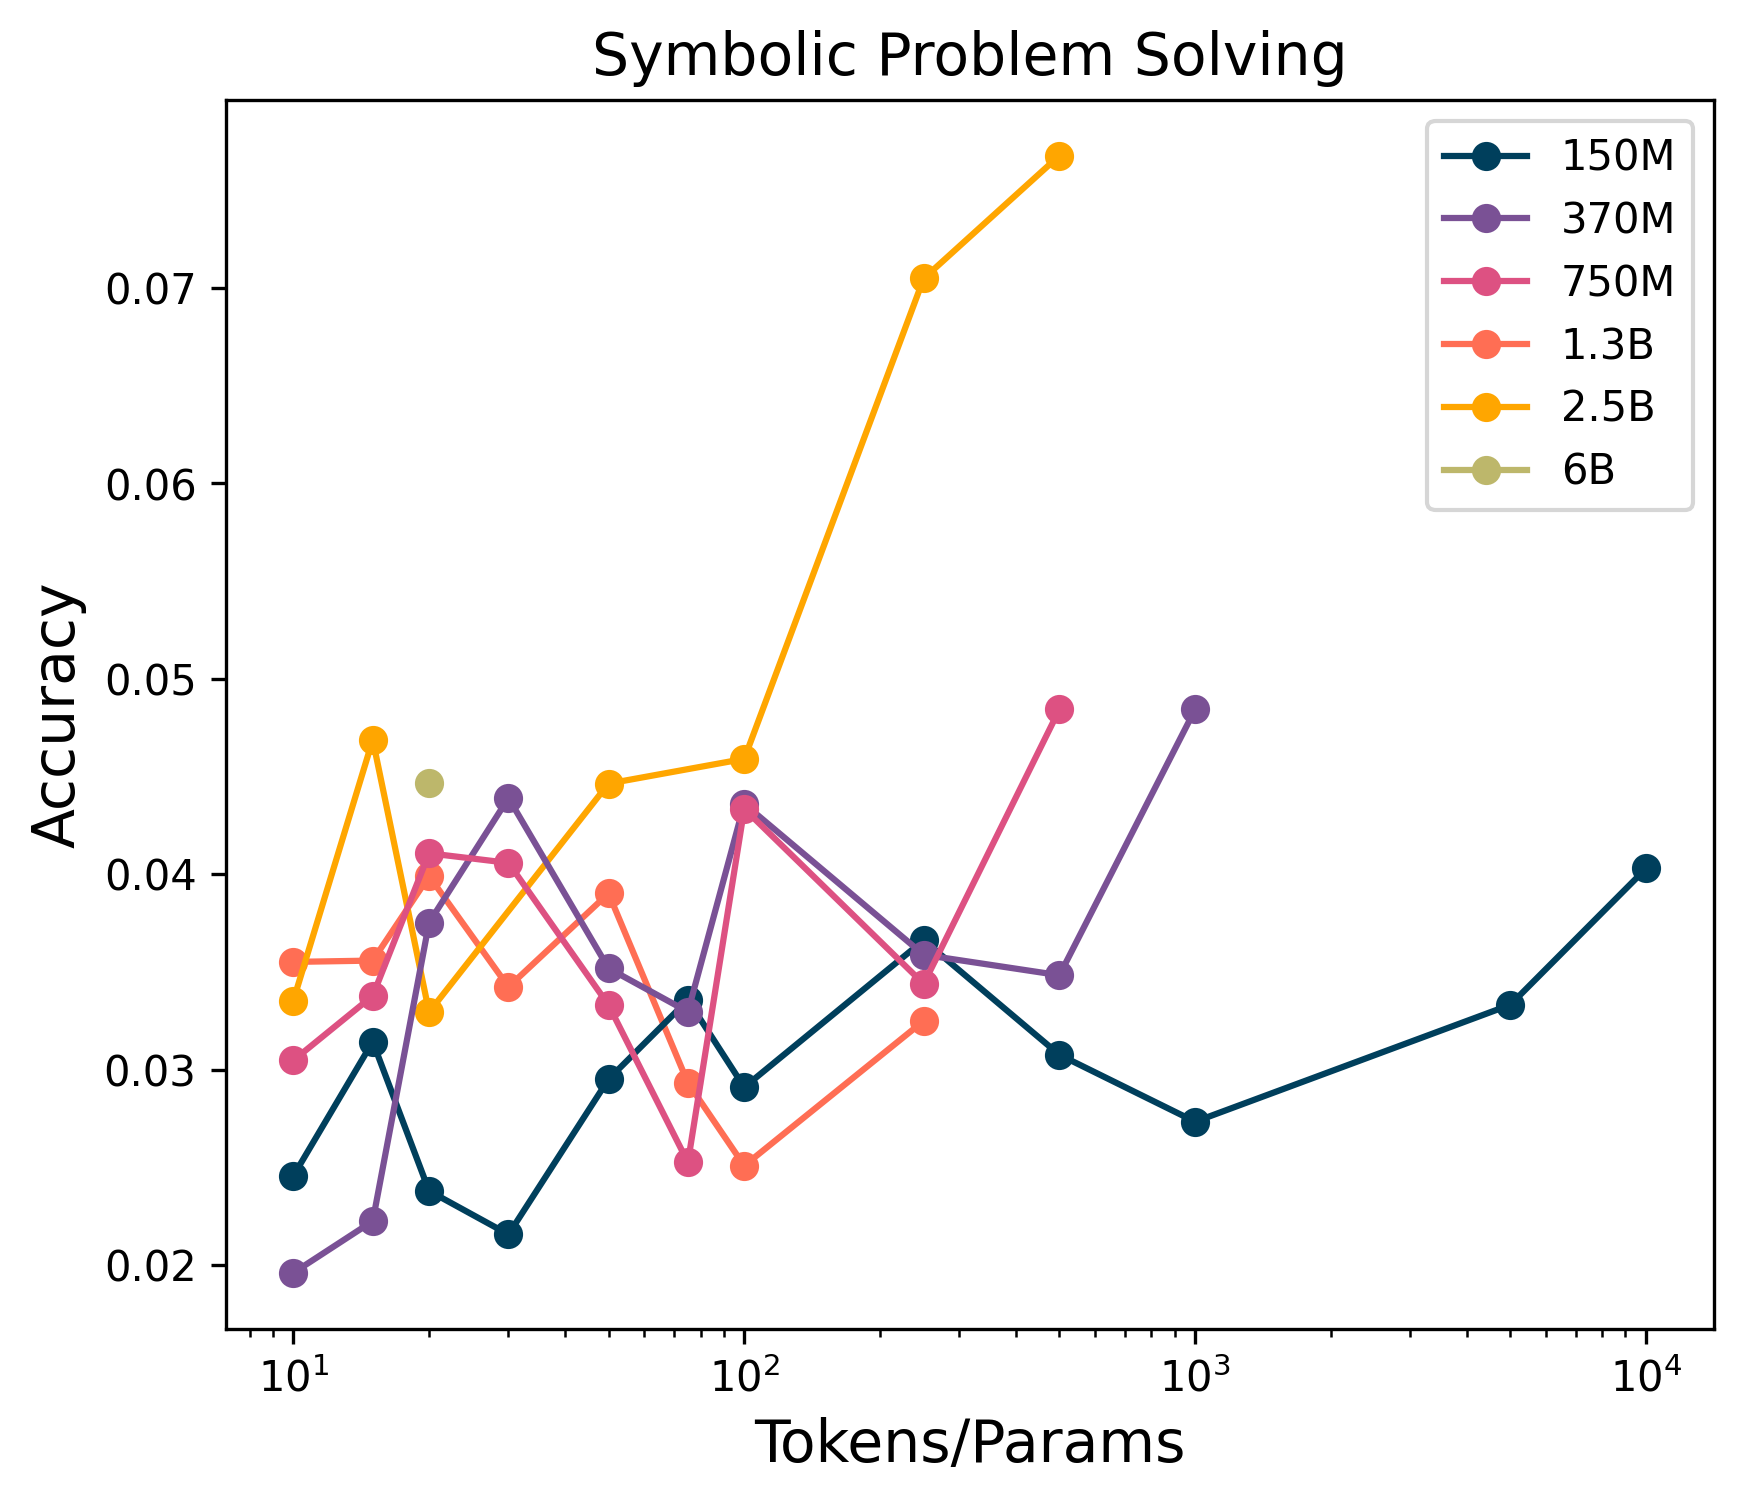
\includegraphics[width=1.00\linewidth]{figs_camera/Symbolic_Problem_Solving_vs_TokensParams.png}
                \caption{}
                \label{fig:symbolicproblemsolving}
        \end{subfigure}
        \caption{Per-category Gauntlet results.}
        \label{fig:gauntletcategories}
\end{figure}




    






